\documentclass[11pt]{report}
\usepackage[utf8]{inputenc}
\usepackage[a4paper, margin=1.2in]{geometry}

\usepackage{listings}
\usepackage{color}
\usepackage{mathtools}
\usepackage{graphicx}
\usepackage{wrapfig}
\usepackage{abstract}

\graphicspath{{diags/}}

\renewcommand{\abstractnamefont}{\normalfont\Large\bfseries}
\renewcommand\bibname{References}

\definecolor{gray}{rgb}{0.5,0.5,0.5}

\lstdefinelanguage{RLamb}{
    morekeywords={let,letregion,in,end,at,void,int},
    literate={->}{\ensuremath{\rightarrow}~}2
             {<=}{\ensuremath{\leq}~}2    {>=}{\ensuremath{\geq}~}2
             {R}{\ensuremath{\rho}}1
             {R1}{\ensuremath{\rho_1}}1   {R2}{\ensuremath{\rho_2}}1
             {R3}{\ensuremath{\rho_3}}1   {R4}{\ensuremath{\rho_4}}1
             {R5}{\ensuremath{\rho_5}}1   {R6}{\ensuremath{\rho_6}}1
             {RH}{\ensuremath{\rho_H}}1   {RL}{\ensuremath{\rho_L}}1
             {A}{\ensuremath{a~}}1        {N}{\ensuremath{n~}}1
             {P}{\ensuremath{p~}}1        {X}{\ensuremath{x~}}1
             {Y}{\ensuremath{y~}}1        {Z}{\ensuremath{z~}}1
             {\('L\)}{\ensuremath{_L}~}1
             {\\:}{\ensuremath{\lambda}}1,
    sensitive=f,
}[keywords,comments,strings]

\lstset{
    language=RLamb,
    aboveskip=3mm,
    belowskip=3mm,
    basicstyle={\small\ttfamily},
    breakatwhitespace=true,
    columns=flexible,
    escapeinside={(@}{@)},
    frame=l,
    keepspaces=true,
    numbers=left,
    numberstyle=\tiny\color{gray},
    showstringspaces=false,
    tabsize=4,
    xleftmargin=4pt
}

\title{Seminar Report Draft}
\author{John C F}
\date{April 2016}

\begin{document}
\begin{titlepage}
    \begin{center}
        \fontfamily{ptm}
        {\LARGE \bfseries Static Methods for Memory Management \par}
        \vspace{\stretch{0.3}}
        { \large \em \fontfamily{pzc} 
            A Seminar Report \\ [.25\baselineskip] 
            submitted in partial fulfillment of the \\ [.25\baselineskip] 
            requirements for the degree of \\ [.25\baselineskip] 
            {\fontfamily{ppl} \bfseries  Master of Technology } \\ [.5\baselineskip] 
            by \par
        }
        \vspace{\stretch{0.1}}
        {\large \bfseries John C F\par}
        \vspace{.25\baselineskip}
        {\large 14305R006}\vspace{\stretch{0.3}}

        {\large Under the guidance of\par}\vspace{.25\baselineskip}
        {\large \bfseries Prof. Amitabha Sanyal \par}

        \vspace{\stretch{0.3}}
        
\includegraphics[width=10em]{iitb-black}

        {\fontfamily{ptm}
            \vspace{\stretch{0.1}}
            {\large Computer Science \& Engineering\\[0.25\baselineskip]
                Indian Institute of Technology Bombay \\[0.25\baselineskip]
                Mumbai 400076  (India) }
            \\[0.5\baselineskip]
            {\large April 2016 \par}
        }
    \end{center}
\end{titlepage}

\begin{abstract}
    Memory management is one of the major concerns when building reasonably complex programs. In this report, we will investigate two static methods of analyzing programs so as to minimize the effort needed at runtime for resource management.
\end{abstract}

\tableofcontents

\chapter{Introduction}

Historically, all memory management was done manually, where the programmer would be supposed to carefully allocate and free memory as needed. This could result in many bugs due to the human-nature of programmers (which is to err!) such as:

\begin{enumerate}
\item Accessing unallocated memory regions (use-after-free, out-of-bounds)
\item Forgetting to free unused memory regions (memory leaks)
\end{enumerate}

Use-after-free behavior usually causes stability issues (the more severe, the better!), but the subtle ones might open up terrible security holes. Minimizing memory leaks is especially crucial for long running programs. In embedded systems, memory might be very limited, and to make matters worse, the operating system may not have process isolation features (virtual memory).

Therefore, due to obvious reasons, automatic memory management techniques were researched. The most commonly used techniques involve a runtime routine which actively scans for allocated but ``stale" memory regions (garbage) and frees them. These techniques are collectively termed Garbage Collection, and it usually involves a per-``object" reference counting along with reachability tracing. Tracing procedure is compute-intensive, as well as it requires that the references don’t change while it does the trace (stop-the-world). Although the tracing routines is infrequently invoked at runtime (when memory usage crosses a certain threshold), it would still incur unacceptable levels of latencies for real-time applications. So the question is: can we do less at runtime and still be safe from memory bugs?

Two major approaches were formulated to address this question:

\begin{itemize}
\item \textit{Regions:} An extended stack-based discipline to support dynamic sized types.
\item \textit{Linear types:} A type system that ensures that objects are used (or consumed) exactly once. Thus simplifying resource management.
\end{itemize}

In chapters that follow, many example programs and associated errors are discussed. All errors under discussion are caught during static analysis.

\chapter{Region Based Memory Management}

\begin{wrapfigure}{r}{0.5\textwidth}
\centering
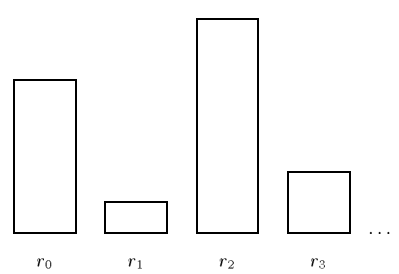
\includegraphics[width=0.5\textwidth]{regions-blocks.png}
\caption{Stack of regions}
\end{wrapfigure}

In this model (as described by Tofte and Talpin\cite{tofterbmm}), the memory is thought of as a stack of regions. And each region can grow indefinitely as values are put into it. All regions are associated with some lexical scope (a code segment) which is responsible for deallocating the whole region when the program exits that scope. The scheme we will discuss involves translation of source language into a region annotated target language using a technique called region inference. The region inference methodology discussed is provably memory safe; that is, values are associated with regions in such a way that there are no dangling pointer dereferences.

It is important to note that regions can only grow and do not shrink -- that is, values can only be put into it, and cannot be individually freed from it. Also, it should be emphasized that, in this scheme, the programmer cannot manage regions, and has no control over which values are put into which regions. Region Inference takes care of all association of values with regions. Before diving into the details of region inference, here’s a small example of the source language and the target language:

\begin{lstlisting}
let X = (2, 3) in (\:Y.(fst X, Y)) end 5
\end{lstlisting}

\noindent which translates to:

\begin{lstlisting}
letregion R4, R5
in letregion R6
   in let X = (2 at R2, 3 at R6) at R4
      in (\:Y.(fst X, Y) at R1) at R5
      end
   end
   5 at R3
end
\end{lstlisting}

\subsection*{Points of note}

\begin{itemize}
\item All values are boxed (live behind a reference). That is, all constants and variables in the program are treated as a reference to the some location (in the heap) managed by regions.
\item \texttt{fst} takes (a reference to) a pair and returns (a reference to) its first element.
\item $e$ \texttt{at} $\rho$ means ``store the value produced by $e$ in the region $\rho$".
\item The only way of introducing and destroying regions is using \texttt{letregion} blocks.
\item Region variables $\rho_1$, $\rho_2$ and $\rho_3$, occurring free in the above code, will contain the final result.
\item The closure (lambda expression) itself is stored at $\rho_5$, which when applied on an argument (binding $y$ to a reference) will store a pair at $\rho_1$ and return (a reference to) that pair.
\item $x$ escapes the \texttt{let} block with the closure (i.e. the closure holds a reference to $x$).
\item Part of $x$ ($3\tt~at~\rho_6$) is deallocated and a dangling pointer is formed (see figure \ref{fig:regions}), but it is safe since it will not be dereferenced.
\item Region variables $\rho_4$ and $\rho_5$ may be bound to the same region.
\end{itemize}

\begin{figure}[h]
\centering
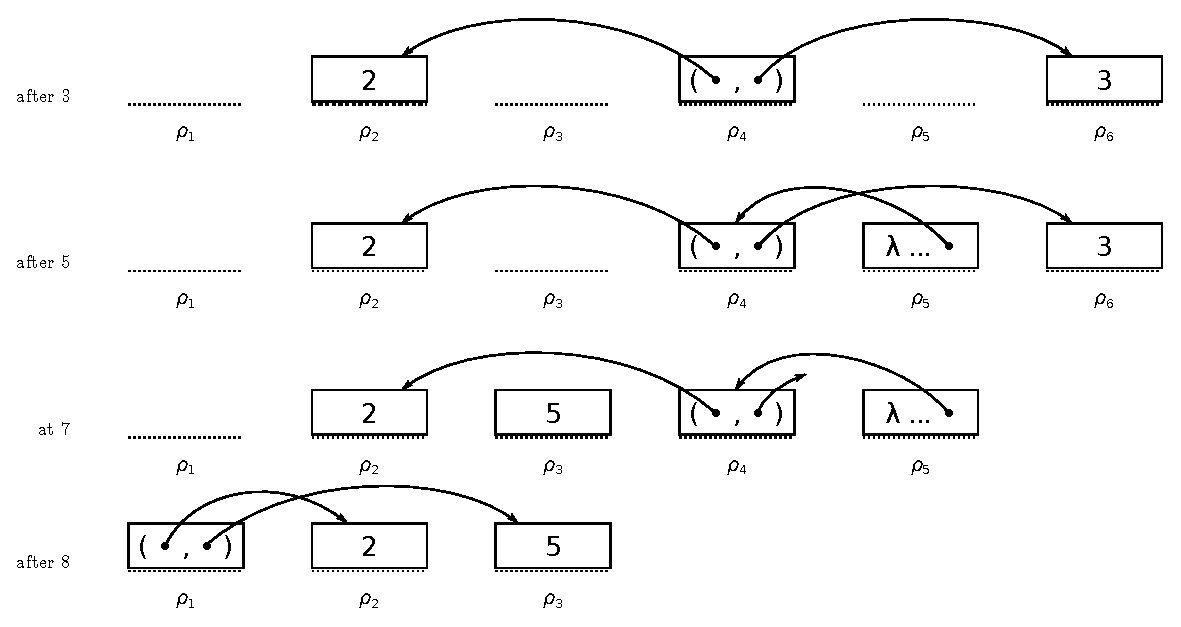
\includegraphics[width=\textwidth]{regions-flow}
\caption{State of regions at various stages of execution}
\label{fig:regions}
\end{figure}

\chapter{Region Inference}

In this chapter, we'll take a detailed look at the translation using the example from before:

\begin{lstlisting}
let x = (2, 3) in (\:Y.(fst X, Y)) end 5
\end{lstlisting}

The most interesting part in the translation was that it was inferred that $x$ escaped the \texttt{let} block as well as that part of $x$ could be thrown away even before the closure was applied! Before we dive into the algorithm, let me give you a rough idea of the type system of the target language.

Below, we will be discussing the type, ``place", and ``effect" of various expressions in the target language. ``$e~::~\tau, \rho~$ w.e. $\epsilon$" is read ``expression $e$ produces a value of type $\tau$ at place $\rho$ with effect $\epsilon$". A place simply means a region; within the scope of our discussion, ``place" and ``region" may be used interchangeably. Effect indicates the set of regions accessed when the expression $e$ is executed. The effect may be empty, or may contain one or more of $\rm get(\rho)$'s or $\rm put(\rho)$'s, which respectively indicate reading a value (involving a dereference) from or writing a new value (involving an allocation) to region $\rho$. We'll use a shorthand of $\rm \{get(\rho_1, \rho_2)\}$ to indicate $\rm \{get(\rho_1), get(\rho_2)\}$.

Let's take a look at how the type scheme (a.k.a polytype) of the built-in \texttt{fst}, which takes in a pair and returns the first element, might be represented in the target language:
\begin{align*}
\forall \rho_0 \rho_1 \rho_2 \forall \alpha_1 \alpha_2. ((\alpha_1, \rho_1) * (\alpha_2, \rho_2), \rho_0) \xrightarrow{\epsilon.\{get(\rho_0)\}} (\alpha_1, \rho_1), \rho'
\end{align*}
$\forall \rho_0 \rho_1 \rho_2$ denotes that the function is region-polymorphic over three region variables, and $\forall \alpha_1 \alpha_2$ denotes that it is type-polymorphic too. ($\mu_1 * \mu_2, \rho)$ denotes the type of a pair stored at region $\rho$, where $\mu_1$ denotes the type and place of the first element, and $\mu_2$ denotes that of the second. $\rm \epsilon.\{get(\rho_0)\}$ above the arrow denotes that, when applying the function, a value from region $\rho_0$ will be read. And finally, $\rho'$ is the place at which this function is stored. For the sake of simplicity, we'll assume that \texttt{fst} is monomorphic to match the context in which it appears, and also ignore the effect of $\rm \{get(\rho')\}$ when \texttt{fst} is applied.

\newpage

\section*{The Algorithm}

The Region Inference algorithm roughly involves the following steps:

\begin{enumerate}
\item Annotate all value-producing expressions with distinct region variables:

\begin{lstlisting}
let x = (2 at R1, 3 at R2) at R3
in (\:Y.(fst X, Y) at R4) at R5
end
5 at R6
\end{lstlisting}

\item Find the type and effect of all expressions (in a bottom-up fashion):
\begin{align*}
\tt fst ::&~ ((int, \rho_1)*(int, \rho_2), \rho_3) \xrightarrow{\epsilon.\{get(\rho_3)\}} (int, \rho_1), \rho'
\\
& \rm ~w.e~ \emptyset
\\
\intertext{The type of \texttt{fst} shown above is the type of \texttt{fst} in that context. ``w.e $\emptyset$" indicates that the expression ``\texttt{fst}", all by itself, does not access any regions. A function reference before being applied to actual arguments does not have any effect.}
\tt (2 ~at~ \rho_1, 3 ~at~ \rho_2) ~at~ \rho_3 ::&~ (int, \rho_1)*(int, \rho_2), \rho_3
\\
& \rm ~w.e~ \tt \{put(\rho_1, \rho_2, \rho_3)\}
\\
\mathtt{fst~} x ::&~ \tt int, \rho_1
\\
& \rm ~w.e~ \tt \{get(\rho_3)\}
\\
\intertext{Note here that the effect of this application is what appeared above the arrow in the type definition of \texttt{fst}. A subtle point to notice is that there is no $\tt get(\rho_1)$ effect. This is because \texttt{fst} only needs to read the value of the pair definition to get the reference to the first value (which is returned without being dereferenced).}
(\mathtt{fst~} x, y) \tt ~at~ \rho_4 ::&~ (int, \rho_1)*(int, \rho), \rho_4
\\
& \rm ~w.e~ \tt \{get(\rho_3), put(\rho_4)\}
\\
\intertext{The most interesting step is up next. The effect of the expression above goes into the type of the closure itself (above the arrow along with an effect variable $\epsilon$). This is the key idea in escape analysis. Even though $\rho_3$ is neither part of the arguments, nor part of the return type, we'll still know that it \textit{will be} accessed by the closure. The effect variable $\epsilon$ is used during monomorphisation of region- (and effect-) polymorphic functions. It is not relevant in this example, and we won't be going into any details of it.}
(\lambda y.(\mathtt{fst~} x, y) \tt ~at~ \rho_4) ~at~ \rho_5 ::&~ (int, \rho_6) \xrightarrow{\epsilon.\{get(\rho_3), put(\rho_4)\}} ((int, \rho_1)*(int, \rho_6), \rho_4), \rho_5
\\
& \rm ~w.e~ \tt \{put(\rho_5)\}
\\
\intertext{Note that since lambda expressions are non-recursive and can only be applied once, the type and place of parameters can be directly inferred from the type and place of actual arguments. This is why $y$ has type $(int, \rho_6)$.}
\tt let~ x = ... ~in~ ... ~end ::&~ (int, \rho_6) \xrightarrow{\epsilon.\{get(\rho_3), put(\rho_4)\}} ((int, \rho_1)*(int, \rho_6), \rho_4), \rho_5
\\
& \rm ~w.e~ \tt \{put(\rho_1, \rho_2, \rho_3, \rho_5)\}
\end{align*}

\item If a region variable occurs free in an expression but does not occur in its type or place (it may occur in the effect), then that expression can be surrounded by a \texttt{letregion} block with that associated region.

Notice in the above expression that $\rho_2$ does not occur in the type and place. Therefore the above block can be wrapped in a \texttt{letregion} involving $\rho_2$.

\begin{lstlisting}
letregion R2
in let x = (2 at R1, 3 at R2) at R3
   in (\:Y.(fst X, Y) at R4) at R5
   end
end
\end{lstlisting}
\begin{align*}
{\rm (above~expression)} ::&~ (int, \rho_6) \xrightarrow{\epsilon.\{get(\rho_3), put(\rho_4)\}} ((int, \rho_1)*(int, \rho_6), \rho_4), \rho_5
\\
& \rm ~w.e~ \tt \{put(\rho_1, \rho_3, \rho_5)\}
\end{align*}

Note that $\rho_2$ is removed from the effect set. This is because, $\rho_2$ is introduced and destroyed within the expression, and the rest of the program need not be aware of it.

\item Repeat steps 2 and 3 for larger scopes:
\begin{align*}
\tt letregion~ \rho_2 ~in~ ... ~end~ 5 ~at~ \rho_6 ::&~ (int, \rho_1)*(int, \rho_6), \rho_4
\\
& \rm ~w.e~ \tt \{get(\rho_3), put(\rho_1, \rho_3, \rho_4, \rho_5, \rho_6)\}
\end{align*}

Notice here that $\rho_3$ and $\rho_5$ does not appear in type and place, and therefore it does not escape out of this expression. And thus by wrapping the whole expression in a \texttt{letregion} introducing those region variables, we’ll get the aforementioned final target code.

\begin{lstlisting}
letregion R3, R5
in letregion R2
   in let x = (2 at R1, 3 at R2) at R3
      in (\:Y.(fst X, Y) at R4) at R5
      end
   end
   5 at R6
end
\end{lstlisting}
\begin{align*}
{\rm (above~expression)} ::&~ (int, \rho_1)*(int, \rho_6), \rho_4
\\
& \rm ~w.e~ \tt \{put(\rho_1, \rho_4, \rho_6)\}
\end{align*}

\end{enumerate}

\section*{Limitations of automatic region inference}

The major limitation of RBMM is that certain values may live longer than needed because it was put into long-living regions. For example, consider this hypothetical case:

\begin{lstlisting}
let X = (read_ints big_file)
in  let Y = len X,
        Z = avg X
    in  long_running Y Z
    end
end
\end{lstlisting}

\noindent Which would be roughly translated to (assume that \texttt{read\_ints[$\rho_1$]} will parse a file and return a list of integers allocated at $\rho_1$):

\begin{lstlisting}
letregion R1
in  let X = (read_ints[R1] big_file)
    in  let ...
        in long_running Y Z end
    end
end
\end{lstlisting}

This would mean that $x$ will remain in memory while \texttt{long\_running} is executed even though it cannot be referenced from it. A resource conscious programmer might want to explicitly free large data structures like those.

The above code could be rewritten in a ``region-friendly" manner as:

\begin{lstlisting}
let (Y, Z) =
    let X = (read_ints big_file)
    in  (len X, avg X)
    end
in  long_running Y Z
end
\end{lstlisting}

\noindent Which will be translated to:

\begin{lstlisting}
let (Y, Z) =
    letregion R1
    in  let X = (read_ints[R1] big_file)
        in ... end
    end
in  long_running Y Z
end
\end{lstlisting}

This refactoring may not always be very straightforward. But this brings us to a major practical issue: the program structure has high influence on how well region inference performs \cite{regionretro}. Therefore, the programmer needs to know how region inference works even though s/he does not directly interact with regions. When the program gets complex, it can be hard to predict region inference.

One other issue with RBMM is concerning tail recursion. It is not always straightforward to do tail call optimization (for instance, it could be inferred that the return value must have the same region as one of the arguments). This can be mitigated by an ad hoc technique called Storage Mode Analysis (during code generation from target language), which resets a region during an allocation if it is found that the values in it are no longer ``live".

Despite the fact that region inference works really well for many programs, it is not always possible to have the optimal reclamation of dead memory. Therefore, in MLKit\cite{mlkitgh} (the first practical language with a complete region inference system), a tracing Garbage Collector (GC) was introduced \cite{elsmanthesis} to minimize memory leaks. It was later proved that a certain type of tracing GC can be safely integrated with region inference \cite{elsmangc}.

\chapter{Simplifying Regions}

In MLKit, the user writes code agnostic of memory management method and the compiler automatically associates each value generating expression with a region of smallest possible lifetime subject to safety constraints.

In Cyclone \cite{grossmanrbmm}, an imperative language which extends C dialect, the user introduces regions and associates values with regions manually, and the compiler simply try to prove safety of those associations or terminates with an error.

Cyclone was an attempt to achieve the following three seemingly conflicting goals:
\begin{itemize}
\item \textit{Safe:} Provide memory safety, type safety, and thread safety
\item \textit{Static:} Safety should be guaranteed at compile-time
\item \textit{Explicit:} The programmer should easily be able to tell (or specify) when objects are allocated and deallocated (how they are managed)
\end{itemize}

By aiming to be Static and Explicit, an implicit goal of Cyclone is to not compromise on performance compared to C.

The main differences of Cyclone compared to MLKit were:

\begin{itemize}
\item \textit{Manual region declaration and annotations:} This made memory management explicit.
\item \textit{Minimal region inference and default annotations:} Region inference was much simplified and limited; instead missing annotations were filled in using default annotation rules wherever possible. This helped reduce the number of annotations required, and easy to translate a piece of code written in C into Cyclone.
\item \textit{Region subtyping:} Since regions are lexical blocks, they cannot partially overlap. Therefore, within a function, regions would have outlives relations between each other. If $\rho_1$ outlives $\rho_2$, then $\rho_1$ is a subtype of $\rho_2$ ($\rho_1$ is $\rho_2$ and more, just as a Cat is an Animal and more). Therefore a pointer \texttt{int *$\rho_1$} (an integer pointer to a value inside $\rho_1$) can be safely typecast to \texttt{int *$\rho_2$}. This is a key idea during region analysis to prove that a program is free of dangling pointer dereferences.
\item \textit{Simple effects:} There are no effect variables, and instead there is a type operator, $\mathtt{regions\_of}(\tau$), which gives the set of regions that occur in $\tau$ (a \texttt{struct} may have multiple pointers to values in various regions). A function, which takes arguments of types $\tau_1$, $\tau_2$, ..., and returns $\tau_0$, is assumed to access regions $\bigcup\limits_{i} \mathtt{regions\_of}(\tau_i)$ when executed.
\end{itemize}

\definecolor{code}{RGB}{80, 80, 80}

\newcommand{\snippet}[1] {\textcolor{code}{\texttt{#1}}}

Let us take a look at an example. Below, \snippet{'L: $\{~...~\}$} indicates introduction of a new region \snippet{L}, and \snippet{new expr} evaluates \snippet{expr}, stores it in the so-called heap region (which is assumed to live forever), and returns a pointer to it. \snippet{rnew$_L$ expr} is similar, but it stores it in the region \snippet{L}. $\rho_L$ is the region variable associated with the region \snippet{L}, and $\rho_H$ is associated with the heap region.

\begin{lstlisting}
void cp(int** pp1, int** pp2) {
    *pp1 = *pp2;    // error
}

void foo(int c) {
    int* x = new 5;
    'L: {
        int* y = rnew('L) 8;
        if (c == 1)
            cp(&x, &y);    // unsafe!
    }
    //read *x
}
\end{lstlisting}

The default annotations try to be as general as possible. Thus the fully verbose version of the above code is:

\begin{lstlisting}
void cp<R1, R2, R3, R4>(int*R1 *R2 pp1, int*R3 *R4 pp2) {
    *pp1 = *pp2;    // but R1 != R3
}

void foo(int c) {
    int*RH x = new 5;
    'L: {
        int*RL y = rnew('L) 8;
        if (c == 1)
            cp(&x, &y);
    }
    //read *x
}
\end{lstlisting}

Thus we should replace $\rho_3$ with $\rho_1$ for \texttt{cp} to type-check. Now, let's consider a safe version of the program:

\begin{lstlisting}
void cp<R1>(int*R1 * pp1, int*R1 * pp2) {
    *pp1 = *pp2;
}

void foo(int c) {
    int*RH x = new 5;
    'L: {
        int*RL y = rnew('L) 8;
        if (c == 1)
            cp(&y, &x);    // safe, but errors! RL != RH
        //read *y
    }
    //read *x
}
\end{lstlisting}

The above program errors because the compiler doesn't ``look" inside \texttt{cp} during the call from \texttt{foo} due to performance reasons, nor does the signature carry enough information to guarantee that the body doesn't do anything unsafe (the assignment could be the other way round). So the only way of satisfying the compiler is to write it inline:

\begin{lstlisting}
void foo(int c) {
    int*RH x = new 5;
    'L: {
        int*RL y = rnew('L) 8;
        if (c == 1)
            y = x;
        //read *y
    }
    //read *x
}
\end{lstlisting}

The language (esp. the compiler) is a lot more complex than how it looks from the discussion up until now. Going into anymore details is beyond scope of this report. A few important areas that we skip are listed below:
\begin{itemize}
\item Unique pointers and many other types of pointers, which provide fine-grained control over memory while still guaranteeing safety.
\item How soundness of a Cyclone program is analysed, using a concept called Linear Capabilities\cite{linearregions}.
\item Existential types and their interaction with regions. This was introduced in order to replace \texttt{void\,*} usage which is not type-safe.
\end{itemize}

The initial design did not provide thread-safety guarantees. But soon an extension was proposed\cite{grossmanthread} to address that. According to this new proposal, each region should maintain a list of threads accessing it at runtime. When a thread exits, it must remove its entry from those lists maintained by the regions it accesses. If a list becomes empty, free the region corresponding to it. Thus access to the list of threads must be protected by locks. These overheads were significant enough that it was never implemented.

In the next chapter, we will discuss an alternative to region based memory management, which avoids such book-keeping of allocated memory chunks at runtime; instead, the variables (or pointers) themselves are responsible for the resources they hold.

\chapter{Linear Type System}

In Linear Type system (as described by Wadler\cite{linearchange}), every object must be used (a.k.a consumed) exactly once. Thus the system can safely reclaim an object's resources after its use. This is a natural way of modeling the real world (and state machines). More concretely, an object, which represents a set of resources (a chunk of memory, an acquired lock, an open socket etc.), is \textit{uniquely} bound to a variable. And the variable must be ``used" exactly once. Next, we will look at how a purely linear typed language might behave using an approximate syntax of Rust, a language which has its roots in Linear Type system (although, Rust is more formally based on a concept called ``External Uniqueness"\cite{externuniq}). Further, we will progressively relax the constraints of Linear Type system and approach the semantics of Rust. In the following example, assume that \texttt{add} and \texttt{print} are built-ins, and \texttt{print} accepts an arbitrary number of parameters:

\begin{lstlisting}
let a = 5;
let b = 6;
let c = add(a, b); // a and b are consumed
print(c); // c is consumed
//print(a, b); // error!
\end{lstlisting}

Since objects are uniquely bound to a variable, we may redefine the meaning of ``consume" in terms of program variables: a variable is said to be consumed when it loses its binding to an object. That does not necessarily mean that the resources held by the object is released right away. Precisely answering when the underlying resource gets released can be difficult. But we can precisely define when a variable is consumed. Below are two rules of consumption:

\begin{enumerate}
\item A variable is consumed when it goes out of scope.\footnote{This makes the ``consume" implicit, and it might be appropriate to call it Affine Typing.}
\item A variable is consumed when it appears in an expression.\footnote{While pattern matching, this may not hold true. Depending on the pattern, the object may be consumed, borrowed (next section), or left untouched (a no-op).}

This means that the variable \texttt{a} gets consumed in all three cases shown below:

\begin{lstlisting}
f(a);
\end{lstlisting}

\begin{lstlisting}
let b = a;
\end{lstlisting}

\begin{lstlisting}
a;
\end{lstlisting}
\end{enumerate}

These rules (almost) enforces Linear Typing, and enables some neat analysis. In particular, spawning a thread involves a function call (and a closure), and multiple variables may get consumed in the process. Thus, objects can be passed between threads without any scope for data race, since there is no aliasing.

But, as you can see, this scheme would be too restrictive and impractical. Thus, Rust introduced \texttt{Copy} types which can \textit{only} get consumed by going out of scope. Whenever a \texttt{Copy} typed variable is accessed, a duplicate copy is created and consumed. All numeric primitives are \texttt{Copy} types in Rust. It is important to note that a ``copy" is not an alias of the original object; it is a separate independent object. For the sake of keeping examples simple, we will consider floating point numbers as non-\texttt{Copy} types.

Now let us see how a linear list would behave (assume that \texttt{get} is a built-in):

\begin{lstlisting}
let a = [1, 3, 5];
//let c = add(get(a, 0), get(a, 2)); // error: a is consumed twice
\end{lstlisting}

To get around this, we could redesign \texttt{get} to return both the original list as well as a copy of the element at the given index:

\begin{lstlisting}
let a0 = [1, 3, 5];
let (a1, b0) = get(a0, 0); // pattern-matched value-binding of a pair
let (a2, b1) = get(a1, 2);
let c = add(b0, b1);
\end{lstlisting}

But what if the elements are not copy-able (e.g. a list of file descriptors)? We could make \texttt{get} reject lists with non-\texttt{Copy} elements, and provide another built-in called \texttt{remove} which works as follows:

\begin{lstlisting}
let a0 = [1.0, 3.0, 5.0];
let (a1, b0) = remove(a0, 0); // a1 = [3.0, 5.0] and b0 = 1.0
let (a2, b1) = remove(a1, 1); // a2 = [3.0] and b1 = 5.0
let c = add(b0, b1);
\end{lstlisting}

This is still too restrictive, and most programs would need to be written in a ``threaded-style" as shown above.

\section*{Borrowing}

Wadler noted that ``it is perfectly safe to have more than one reference to a value temporarily, as long as only one reference exists when the update is performed"\cite{linearchange}. This is the key idea behind the concept of Borrowing in Rust. Thus we will extend the rules of consumption to accommodate this:

\begin{enumerate}
\setcounter{enumi}{2}
\item A variable is not consumed in an expression when it is preceded by a borrow operator (discussed next).
\item A variable must not be consumed when a borrow is in effect.
\end{enumerate}

\texttt{\&} is a borrow operator. Below, \texttt{\&a} denotes borrow of \texttt{a}. Technically, \texttt{b} is a pointer to the value \texttt{8.0}, but the responsibility of the underlying resource rests solely on \texttt{a}. And \texttt{b} is called a (shared) reference.

\begin{lstlisting}
let a = 8.0;
let b = &a;
let c = add(3.0, a); // error: a is borrowed
\end{lstlisting}

\newpage

\noindent Points of note:
\begin{itemize}
\item \texttt{b} is a read-only view of \texttt{a}.
\item There can be multiple shared references at the same time.
\item Shared references are also \texttt{Copy} types. So \texttt{b} will not get consumed (and consequently the borrow does not end) until it goes out of scope.
\end{itemize}

In the next example, assume that \texttt{add\_ref} takes a shared reference as the second argument and adds its value to the first, then returns the result.

\begin{lstlisting}
let a = 8.0;
{   // introduce a new scope
    let b = &a;
    let c = add_ref(3.0, b);
}   // borrow ends
let d = add(3.0, a);
\end{lstlisting}

Now, since it is safe to update an object when it is not aliased (i.e. no borrow is in effect), another kind of borrow was introduced: a ``mutable borrow" which allowed in-place updates. \texttt{\&mut} is the operator for mutable borrowing. In the next example, assume that \texttt{add\_mut} takes in a mutable reference and updates it in-place.

\begin{lstlisting}
let mut a = 8.0; // mut marks `a' as in-place updateable
add_mut(&mut a, 4.0); // a mutable reference is created and consumed
print(a); // prints 12.0
\end{lstlisting}

An object's mutability is strictly unique. That is, an object cannot be mutably borrowed while another borrow (mutable or not) is in effect and vice versa. To see why they should be unique, consider the following example (assume that square brackets introduces a dynamic list; \texttt{truncate} resizes the list to a new length; and \texttt{print} will automatically read the value pointed to by a reference that is passed to it):

\begin{lstlisting}
let a = [1.0, 3.0, 5.0];
let b = get_ref(&a, 2); // b = &a[2], indirectly borrowing `a'
truncate(&mut a, 1); // drop the last two elements
print(b); // dangling pointer dereference
\end{lstlisting}

The above program will not compile, of course. This means that Rust provides two guarantees:

\begin{itemize}
\item If you hold a shared reference (\texttt{\&T}), you are guaranteed that it will not become invalid as long as you hold it.\footnotemark
\item If you hold a mutable reference (\texttt{\&mut T}), you are guaranteed that you are having \textit{exclusive access} to it. Thus, even destroying (or rewriting) a part of it will not affect any other references that are alive at that moment.
\end{itemize}
\footnotetext{Rust does not guarantee that it will not be mutated because certain types may have ``internal mutability". Examples include wrappers which provide dynamic borrow-checking and mutual exclusion among others. But Rust guarantees that such mutations will not cause \textit{Undefined Behavior}.}

Since a mutable reference is non-\texttt{Copy}, ideally, the borrow should end the first time it is consumed and the ``lender" (or ``owner") variable should become accessible. But this is not the case because keeping track of borrows through flow analysis can be inefficient and difficult to prove correctness. And this is where Rust meet Regions. Rust uses an algorithm based on Region Inference to keep track of borrows.

All borrows are associated with a lexical scope called the ``lifetime of borrow", and it represents the span of effect of that borrow. The reason for associating a lexical scope is so that lifetimes can have subtype (or outlives) relation between each other (no partial overlaps). This means that the following code is invalid:

\begin{lstlisting}
let mut a = 8.0;
let b = &mut a;
if condition {
    add_mut(b, 2.0); // consume b(@\footnotemark@), but borrow does not end!
    let c = &mut a; // error: a is borrowed
}
\end{lstlisting}
\footnotetext{This is not exactly true since Rust automatically converts it to a reborrow (discussed later). To keep things explicit, we will ignore that feature of Rust. By the way, \texttt{b;} \textit{will} consume \texttt{b} in Rust.}

The lifetime of a reference is upper-bounded by the scope of the owning variable. And inside the lifetime of the borrower, the object cannot be consumed (consumption rule 4).

\begin{lstlisting}
let b; // defer initialization(@\footnotemark@)
{
    let a = 8.0;
    b = &a; // error: scope of a is too small
}
\end{lstlisting}
\footnotetext{\texttt{b} need not be marked as mutable, because through data-flow analysis, Rust can verify that \texttt{b} is not accessed while uninitialized, and that it will be initialized exactly once.}

\subsection*{Reborrowing}

Since mutable references cannot be \texttt{Copy}, we can't do the following:

\begin{lstlisting}
fn add_six(b: &mut u32) {
    add_mut(b, 4.0); // consume b
    //add_mut(b, 2.0); // error: b was consumed
}
\end{lstlisting}

\noindent Therefore, Rust provides a mechanism called ``reborrowing":

\begin{lstlisting}
fn add_six(b: &mut u32) {
    add_mut(&mut *b, 4.0); // reborrow and consume
    add_mut(b, 2.0); // ok
}
\end{lstlisting}

\noindent But of course, reborrowing does \textit{not} allow aliasing mutability:

\begin{lstlisting}
let mut a = 8.0;
let b = &mut a;
{
    let c = &mut *b; // reborrow
    //add_mut(b, 2.0); // error: b is reborrowed
}
add_mut(b, 2.0); // ok
\end{lstlisting}

\noindent That is, every reborrow supersedes the previous borrow as long as it exists (in-scope).

\section*{Lifetime}

In Rust, \textit{concrete} lifetimes are hidden from the programmer except the so-called \texttt{'static} which indicates forever-lifetime. The programmer is supposed to play with abstract lifetimes, as parameters in a function or type. For example, the above \texttt{add\_six} function may be rewritten as follows with explicit lifetime annotation:

\begin{lstlisting}
fn add_six<'a>(b: &'a mut u32) {
    add_mut(&mut *b, 4.0);
    add_mut(b, 2.0);
}
\end{lstlisting}

The lifetime parameter \texttt{'a} is kept abstract, even during analysis of the above function, with the assumption that \texttt{'a} outlives the entire scope of the function. Do note that, similar to Cyclone, Rust does not do whole-program lifetime inference. All inference takes place at an intra-procedural level, and therefore the programmer is required to insert explicit lifetime annotations wherever a set of default annotation rules is not appropriate. Thus, at the site of a function call, the compiler need to only check for inconsistencies with the given lifetime constraints of the function signature. We will take a closer look at this, but first, let us take a look at how the compiler assigns concrete lifetimes to a simple program:

\begin{lstlisting}
let mut a = 8.0;
{
    let b = &mut a;
    add_mut(&mut *b, 6.0);
    add_mut(b, 2.0);
}
\end{lstlisting}

\noindent This is viewed by the compiler as:

\begin{lstlisting}
'x: {
    let mut a = 8.0;
    'y: {
        let b = &'y mut a;
        'z: {
            add_mut(&'z mut *b, 6.0);
        }
        add_mut(b, 2.0);
    }
}
\end{lstlisting}

Note that the short scope of \texttt{'z} indicate that the reborrow is short-lived, after which \texttt{b} can be used (i.e. \texttt{b} becomes live). It is worth emphasizing that scopes \textit{cannot} be assigned concrete names by the programmer, and used in reference lifetimes, as shown above.

Now, let's try a slightly more complex program involving two functions:

\begin{lstlisting}
fn max_ref<'a>(x: &'a u32, y: &'a u32) -> &'a u32 {
    if *a > *b { // (@\footnotemark@)
        return a;
    } else {
        return b;
    }
}
\end{lstlisting}
\footnotetext{Yes, Rust has the dereference operator \texttt{*}, but we will not go into the details of its semantics.}

\begin{lstlisting}
fn main() {
    let u = 8;
    let ur = &u;
    {
        let v = 4;
        let vr = &v;
        let mr = max_ref(ur, vr);
        print(mr);
    }
}
\end{lstlisting}

The compiler will view the \texttt{main} function as follows:

\begin{lstlisting}
'a: {
    let u = 8;
    'b: {
        let ur = &'b u;
        'c: {
            let v = 4;
            'd: {
                let vr = &'d v;
                'e: {
                    let mr = max_ref(ur, vr);
                    print(mr);
                }
            }
        }
    }
}
\end{lstlisting}

Note that \texttt{ur} and \texttt{vr} have different associated lifetimes. When the lifetime constraints (such as lifetime equality assertion) does not match that of the actual arguments, the compiler tries to make them match subject to a set of variance rules. In the above case, one of the variance rules states that \texttt{\&'a T} is covariant w.r.t both \texttt{'a} and \texttt{T}. It means that the compiler is free to shrink the lifetime of \texttt{ur} to match that of \texttt{vr}.

Thus the type of \texttt{mr} will be \texttt{\&'d u32}. There is a catch: the reference returned by \texttt{max\_ref} effectively borrows both the arguments, due to the lifetime-equality assertion between the input parameters and the output. Consequently, \texttt{max\_ref(ur, vr)} cannot escape beyond the scope of \texttt{'c}, even though the actual reference returned is \texttt{\&u}.

Finally, let us look at the Rust-equivalent of the Cyclone-examples we discussed.

\begin{lstlisting}
fn cp<'a>(pp1: &mut &'a i32, pp2: &&'a i32) {
    *pp1 = *pp2;
}

fn foo(c: i8) {
    let i = 5;
    let mut x = &i;
    {
        let j = 8;
        let y = &j;
        if c == 1 {
            cp(&mut x, &y); // unsafe! doesn't compile!
        }
    }
    //read *x
}
\end{lstlisting}

\noindent Here is its safe version:

\begin{lstlisting}
fn cp<'a>(pp1: &mut &'a i32, pp2: &&'a i32) {
    *pp1 = *pp2;
}

fn foo(c: i8) {
    let i = 5;
    let x = &i;
    {
        let j = 8;
        let mut y = &j;
        if c == 1 {
            cp(&mut y, &x); // ok!
        }
        //read *y
    }
    //read *x
}
\end{lstlisting}

\noindent Points of note:
\begin{itemize}
\item In the function definition, the inner lifetimes of both references \texttt{pp1} and \texttt{pp2} are annotated to be the same. When there is such an assertion of lifetime equality and the lifetimes in the actual arguments differ, the compiler tries to shrink all bigger lifetimes to match the smallest one, subject to a set of variance rules.
\item \texttt{\&T} is covariant w.r.t \texttt{T} but \texttt{\&mut T} is invariant w.r.t \texttt{T}. Therefore, in the former example, the inner lifetime of \texttt{\&mut x} is not shrunk to match that of \texttt{\&y} (which would be unsafe), but in the latter example, the inner lifetime of \texttt{\&x} is shrunk to match that of \texttt{\&mut y}.
\end{itemize}

These concepts of ownership (linear typing) and lifetimes only exist at compile-time, and therefore no region-management is required at runtime.

Rust provides type abstraction and polymorphism via its ``trait-based" type system. Traits are similar to Haskell type classes or Java interfaces. Rust's type system (traits + ownership + lifetimes) is powerful enough to enforce thread-safety constraints without the compiler having special knowledge about threads. A discussion on traits is beyond the scope of this report.

\chapter*{Conclusion}
\addcontentsline{toc}{chapter}{Conclusion}

In our short survey of literature on provably safe methods to manage memory, we found that seemingly unrelated concepts can be mixed together to create very powerful, efficient, and practical tools that provide strong safety guarantees as well as allow fine-grained resource management.

\begin{thebibliography}{4}
\addcontentsline{toc}{chapter}{Bibliography}
\bibitem{tofterbmm}
Mads Tofte and Jean-Pierre Talpin. \textit{Region-Based Memory Management.} In Information and Computation 132(2), pages 109-176. 1997.

\bibitem{regionretro}
Mads Tofte, Lars Birkedal, Martin Elsman, and Niels Hallenberg. \textit{A Retrospective on Region-Based Memory Management.} Higher-Order and Symbolic Computation (HOSC). 17(3): 245-265, September 2004, Copyright © 2004 Kluwer Academic Publishers.

\bibitem{mlkitgh}
Public source code repository: \textit{https://github.com/melsman/mlkit}

\bibitem{elsmanthesis} 
Martin Elsman. \textit{Program Modules, Separate Compilation, and Intermodule Optimisation.} PhD thesis. Revised. Department of Computer Science, University of Copenhagen. January 1999.
 
\bibitem{elsmangc} 
Martin Elsman. \textit{Garbage Collection Safety for Region-based Memory Management.} In Proceedings of ACM SIGPLAN Workshop on Types in Language Design and Implementation (TLDI’03). New Orleans, Louisiana, USA. January 2003.

\bibitem{grossmanrbmm} 
Grossman, Dan, et al. \textit{Region-based memory management in Cyclone.} ACM Sigplan Notices. Vol. 37. No. 5. ACM, 2002.

\bibitem{linearregions}
Fluet, Matthew, Greg Morrisett, and Amal Ahmed. \textit{Linear regions are all you need.} In Programming Languages and Systems, pp. 7-21. Springer Berlin Heidelberg, 2006.

\bibitem{grossmanthread}
Grossman, Dan. \textit{Type-Safe Multithreading in Cyclone.} ACM Workshop on Types in Language Design and Implementation, pages 13–25, New Orleans, LA, January 2003.

\bibitem{linearchange}
Wadler, Philip. \textit{Linear types can change the world.} IFIP TC. Vol. 2. 1990.

\bibitem{externuniq}
Clarke, Dave, and Tobias Wrigstad. \textit{External uniqueness is unique enough.} In ECOOP 2003–Object-Oriented Programming, pp. 176-200. Springer Berlin Heidelberg, 2003.

\end{thebibliography}

\end{document}
